\documentclass[twocolumn,linenumbers]{aastex701}

\newcommand{\Msun}{M_\odot}
\newcommand{\Etor}{E_{\rm tor}}
\newcommand{\Epol}{E_{\rm pol}}
\newcommand{\Mch}{M_{\rm Ch}}
\newcommand{\bmin}{\beta_{\rm min}}

\shorttitle{Magnetic support versus stable geometry}
\shortauthors{de Lima et al.}

\begin{document}

\title{Magnetic Support and Stable Field Geometry Are Mutually Exclusive
in Super-Chandrasekhar White Dwarfs}

%% Coauthors alphabetical by surname after the first author, the standard
%% convention. AASTeX 7 requires an email for every author.
\author[0000-0003-1718-3838]{Rafael C. R. de Lima}
\affiliation{Departamento de F\'isica, Centro de Ci\^encias Tecnol\'ogicas,
Universidade do Estado de Santa Catarina, Joinville, SC, Brazil}
\email{rafael.lima@udesc.br}

%% TODO(Laura): affiliation. The correspondence only gives "Chile" and a
%% personal address; please replace both lines.
\author{Laura M. Becerra}
\affiliation{TODO --- affiliation to be supplied by the author}
\email{laura.marcela.becerra@gmail.com}

\author{Banibrata Mukhopadhyay}
\affiliation{Department of Physics, Indian Institute of Science,
Bengaluru 560012, India}
\email{bm@iisc.ac.in}

\author{Jorge A. Rueda}
\affiliation{ICRANet and Dipartimento di Fisica e Scienze della Terra,
Universit\`a di Ferrara, Via Giuseppe Saragat 1, 44122 Ferrara, Italy}
\email{jorge.rueda@icra.it}

\author{Zenia Zuraiq}
\affiliation{Department of Physics, Indian Institute of Science,
Bengaluru 560012, India}
\email{zeniazuraiq@iisc.ac.in}

\begin{abstract}

Equilibrium models of magnetized white dwarfs above the Chandrasekhar limit
support the extra mass with an ordered interior field carrying a substantial
fraction of the gravitational binding energy. We ask whether such a star can
carry that field at all, and whether the field can be given the mixed
poloidal--toroidal geometry that is the only one known to be dynamically
stable. Using self-consistent-field equilibria with a Grad--Shafranov
poloidal component and a confined toroidal component, we survey
$1.8\times10^{3}$ configurations spanning central density, field strength,
field localization, and rotation. We find a ceiling on the confined toroidal
field that the star can hold: $\Etor/|W| \le 0.0101$, essentially independent
of central density over a decade and converged to $0.01\%$ between
$129^2$ and $257^2$ meshes. The equilibrium literature requires
$\Etor/|W| \simeq 0.203$, twenty times more. A field the star can hold is
worth $+0.017\,\Msun$, about one per cent, and the mass frontier converges to
$\Mch$ from below without crossing it, terminating at neutronization. Adding
differential rotation removes the mass restriction but not the field ceiling:
configurations above the Chandrasekhar mass with comparable poloidal and
toroidal energies exist, reaching $2.13\,\Msun$ at the edge of the comparable
band and $1.65\,\Msun$ well inside it, but their mass is rotational and their
field still carries only $\sim 1\%$ of the virial. Three-dimensional ideal-MHD evolution of the
configuration the literature specifies shows an $m=1$ instability removing
$98\%$ of the magnetic energy within a few Alfv\'en times while leaving the
field ordered and axisymmetric: what the star cannot keep is the amplitude,
not the geometry. We further show that the stable
mixed configuration cannot be evolved in a domain-filling code at accessible
cost: comparable poloidal energy implies an exterior dipole of
$\sim10^{11}$--$10^{12}$~G, which no affordable ambient medium can confine.
We argue that super-Chandrasekhar white dwarfs, if they exist, are
rotationally supported objects in which the magnetic field is a passenger
rather than the support.

\end{abstract}

\keywords{White dwarfs (1799) --- Stellar magnetic fields (1610) ---
Magnetohydrodynamics (1964) --- Stellar rotation (1629) ---
Type Ia supernovae (1728)}

\section{Introduction} \label{sec:intro}

%% TODO(RL): expand with the SN Ia progenitor motivation and the observational
%% situation for over-luminous events; the technical framing is below.

The possibility that a white dwarf can exceed the Chandrasekhar mass if it is
strongly magnetized has been developed over the last decade into a
programme of equilibrium models
\citep[e.g.][]{subramanian2015,gupta2020,deb2022}. The construction is
consistent within its own assumptions: a sufficiently strong ordered interior
field contributes pressure and tension that support mass beyond what electron
degeneracy alone can hold, and sequences of such equilibria reach
$2$--$2.3\,\Msun$ for interior fields of a few times $10^{13}$~G.

Two things are absent from that programme, and they are connected.

The first is dynamics. The models are stationary equilibria; none has been
evolved. This matters because the field geometries the sequences use --- either
purely toroidal or purely poloidal --- are precisely the two that linear
theory says are unstable. \citet{braithwaite2006} showed that a stable
stellar field requires poloidal and toroidal components of \emph{comparable}
energy, the twisted-torus configuration anticipated by \citet{prendergast1956};
both pure branches are unstable, the toroidal one to the $m=1$ Tayler kink.
The twisted torus does not appear anywhere in the super-Chandrasekhar white
dwarf literature.

The second is the question of whether the star can hold the field it is given.
A field that supports mass necessarily carries a large fraction of the
binding energy, and therefore a magnetic pressure comparable to the gas
pressure somewhere in the star. Where the plasma $\beta = P_{\rm gas}/P_{\rm
mag}$ falls below unity, the field dominates the pressure that the
non-magnetic equation of state used to build the equilibrium was supplying,
and the construction is inconsistent with itself.

This paper addresses both. Section~\ref{sec:methods} describes the equilibrium
construction and the criteria we impose. Section~\ref{sec:ceiling} establishes
a ceiling on the confined toroidal field a white dwarf can hold and shows that
the mass frontier it permits saturates at $\Mch$. Section~\ref{sec:rotation}
adds differential rotation and shows that super-Chandrasekhar twisted-torus
configurations do exist, but that their mass is rotational.
Section~\ref{sec:3d} presents three-dimensional evolution of the literature's
configuration and of the stable alternative. Section~\ref{sec:discussion}
draws out what this implies for the programme, and
Section~\ref{sec:limitations} states the limitations, several of which are
severe and are placed there deliberately rather than at the end.

\section{Methods} \label{sec:methods}

\subsection{Equilibrium construction}

%% TODO(RL): cite the SCF scheme and the code description properly.

Equilibria are computed with a self-consistent-field scheme in the manner of
\citet{hachisu1986}, on a spherical $(r,\theta)$ grid without assumed
equatorial symmetry. The equation of state is the zero-temperature degenerate
electron gas of \citet{chandrasekhar1935} with $\mu_e = 2$, which is also the
equation of state used in the three-dimensional evolution, so that the initial
condition is in genuine equilibrium under the same physics that evolves it.

The toroidal field is self-consistent, entering the Bernoulli integral through
its own term, with $B_\phi \propto \rho\varpi$. The poloidal field follows
from the Grad--Shafranov equation
\begin{equation}
\Delta^{*} u = -4\pi \varpi^{2} \rho\, \mu(u),
\end{equation}
where the arbitrary function $\mu$ controls how the current is distributed.
The choice $\mu = \mathrm{const}$, used by essentially all earlier work,
produces a vacuum dipole exterior. Following \citet{fujisawa2012} we also use
the negative-power form $\mu(u) \propto (u+\epsilon)^{m}$, which concentrates
current toward the axis and enlarges the closed-field-line region; $m=0$
recovers the constant case. Because $\mu$ depends on $u$ the equation is
nonlinear and is solved by under-relaxed iteration.

A twisted torus requires the toroidal field to vanish on every field line that
reaches the vacuum, so the toroidal component is confined to the closed-line
region, with the profile $B_\phi \propto w^{\zeta}/\varpi$ where
$w$ is the normalized flux inside that region. This confinement is the
physical content of the twisted-torus requirement and, as we show below, it is
also what limits the field the star can hold.

Rotation follows the $j$-constant law
$\Omega(\varpi) = \Omega_c A^2/(A^2+\varpi^2)$ with $A$ set to the equatorial
radius of the non-rotating reference star at the same central density, and
$\Omega_c$ quoted as a fraction of that reference's Keplerian frequency.

\subsection{The four criteria} \label{sec:criteria}

A configuration is counted as viable only if it satisfies all of:

\begin{enumerate}
\item $M > \Mch = 1.44\,\Msun$ for $\mu_e = 2$: it is super-Chandrasekhar at
      all.
\item $\bmin \ge 1$, where $\bmin$ is the minimum of
      $P_{\rm gas}/P_{\rm mag}$ over the region $\rho > 10^{6}$~g~cm$^{-3}$:
      the star can hold its own field. We stress that this is a consistency
      condition on the construction, not a proof of dynamical stability.
\item $0.1 < \Etor/\Epol < 10$: the poloidal and toroidal energies are
      comparable, which is the \citet{braithwaite2006} stable branch. Both
      pure branches are excluded by this criterion, as they should be.
\item $T/|W| < 0.14$ and no mass shedding: the rotation is one the star can
      keep. The threshold is the secular bar mode; the dynamical one is
      $0.27$. A star held up by rotation it cannot retain is not a result.
\end{enumerate}

Criterion (iv) is inactive for the non-rotating survey of
Section~\ref{sec:ceiling} and becomes the binding constraint in
Section~\ref{sec:rotation}.

\subsection{Three-dimensional evolution}

Evolution uses CASTRO \citep{almgren2010} with ideal MHD, constrained
transport, and the HLLD Riemann solver on a single-level Cartesian grid, with
monopole self-gravity and the same zero-temperature equation of state.
Equilibria are exported as a vector potential so that $\nabla\cdot\mathbf{B}$
is zero to round-off on the target mesh; the reconstruction is verified before
any run, with relative $|\nabla\cdot\mathbf{B}| < 10^{-12}$ and curl errors
below $5\times10^{-2}$.

\section{The field a white dwarf can hold} \label{sec:ceiling}

%% Numbers in this section: investigations/tt_sweep.csv (1250 rows, 50 grid
%% points) and tt_sweep_hidens.csv (600 rows, 24 off-grid points).

\subsection{A ceiling independent of central density}

We first ask, with rotation switched off, how much confined toroidal field a
white dwarf of given central density can carry while satisfying $\bmin \ge 1$.
Figure~\ref{fig:ceiling} gives the answer.

\begin{figure}
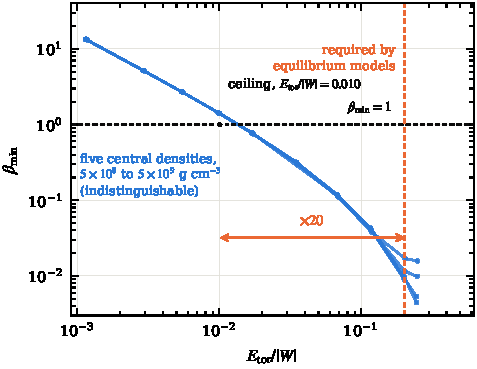
\includegraphics[width=\columnwidth]{figures/fig_ceiling.pdf}
\caption{The minimum plasma $\beta$ over the stellar interior against the
energy the confined toroidal field is asked to carry, for five central
densities between $5\times10^{8}$ and $5\times10^{9}$~g~cm$^{-3}$. Each curve
is the envelope over the poloidal shape parameters, that is the best $\beta$
the star achieves at that field strength. The five curves are
indistinguishable: the ceiling is a property of the confinement rather than of
the star. The star holds its field only above the dashed line, which places
the ceiling at $\Etor/|W| = 0.010$, a factor of twenty below the value the
super-Chandrasekhar equilibrium models require.
\label{fig:ceiling}}
\end{figure}

The mass that such a field buys is $+0.013$ to $+0.017\,\Msun$, between one
and two per cent, and the maximum $\Etor/|W|$ the star holds is
$0.0098$--$0.0101$ across a full decade in central density: the ceiling barely
moves. For comparison, the configuration that reaches $2.007\,\Msun$ at
$\rho_c = 10^{9}$~g~cm$^{-3}$ in the standard construction carries
$\Etor/|W| = 0.203$ --- a factor of twenty above the ceiling.

The reason the ceiling is so low is geometric rather than energetic. A twisted
torus requires the toroidal field to live only inside the closed-line region,
which is $37$--$45\%$ of the stellar volume depending on the localization
exponent $m$. Forcing the energy that supports the mass into that fraction of
the volume raises the peak field where it lives, and $\beta$ fails in a shell
near $\rho \sim 10^{6}$~g~cm$^{-3}$ before the poloidal component has been
introduced at all. We verified this directly: at fixed $\Etor/|W| = 0.203$,
$\bmin = 6\times10^{-3}$ and is identical to three digits across three decades
of poloidal amplitude. It is the confinement, not the mixed geometry, that
breaks $\beta$.

\subsection{The frontier saturates at the Chandrasekhar mass}

Because the ceiling rises slowly with central density while the field-free
mass rises toward $\Mch$, the two effects nearly cancel. Extending the survey
to $\rho_c = 1.8\times10^{10}$~g~cm$^{-3}$, just below the neutronization
threshold of $1.94\times10^{10}$~g~cm$^{-3}$ for $\mu_e = 2$, the heaviest
configuration holding its own confined toroidal field is $1.4387\,\Msun$, and
the margin to $\Mch$ halves at each density step: $+0.0123$, $+0.0062$,
$+0.0026$, $+0.0013\,\Msun$.

\begin{figure}
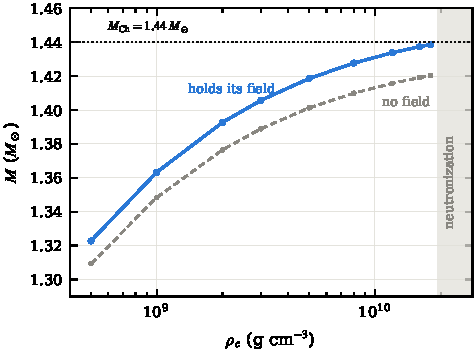
\includegraphics[width=\columnwidth]{figures/fig_frontier.pdf}
\caption{The heaviest configuration that holds its own confined toroidal field
(solid) against central density, with the field-free sequence (dashed) for
scale. The separation between the curves is what the field buys, between
$0.013$ and $0.017\,\Msun$. The upper curve approaches the Chandrasekhar mass
without reaching it, and the sequence terminates at the neutronization
threshold (shaded) rather than at a field limit.
\label{fig:frontier}}
\end{figure}

The frontier therefore converges to the Chandrasekhar mass from below and does
not cross it. This is a stronger statement than ``well below'': a magnetically
supported twisted torus saturates \emph{at} the limit that degeneracy alone
already provides. Restricted to the comparable-energy band, the heaviest such
configuration is $1.4245\,\Msun$.

\section{With rotation: the configuration exists} \label{sec:rotation}

%% Numbers: investigations/tt_rotating.csv (540 rows, 75 points) and
%% investigations/max_mass_frontier.py.

The exclusion of Section~\ref{sec:ceiling} is about the \emph{source} of the
mass, not about twisted tori. Repeating the survey with differential rotation,
$40$ of $540$ configurations satisfy all four criteria simultaneously.

Mass and comparability are not independent: both rise with rotation, so the
$\Etor/\Epol$ criterion binds before the secular bar mode does. The object is
therefore a curve rather than a point, and Figure~\ref{fig:tradeoff} and Table~\ref{tab:tradeoff} give it.
A single quoted maximum would be fragile --- the heaviest configuration sits at
$\Etor/\Epol \simeq 10$, and whether it falls inside the band depends on where
the edge is drawn, which is a convention rather than a physical boundary.

\begin{figure}
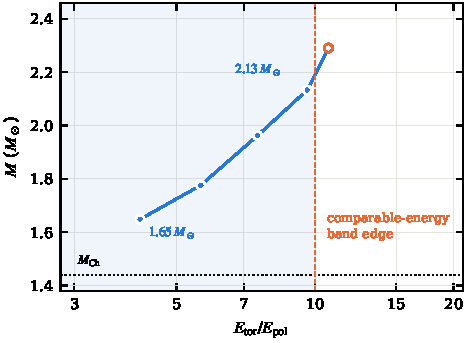
\includegraphics[width=\columnwidth]{figures/fig_tradeoff.pdf}
\caption{Mass against the ratio of toroidal to poloidal energy along the
rotating sequence, with $\bmin = 1$ imposed at every point. Both quantities
rise together with rotation, so criterion (iii) binds before the secular bar
mode does; the open symbol is the configuration that falls outside the
comparable band. Shading marks the band. The heaviest configuration satisfying
every criterion is $2.13\,\Msun$, and a configuration sitting well inside the
band rather than at its edge still carries $1.65\,\Msun$, $14\%$ above the
Chandrasekhar limit.
\label{fig:tradeoff}}
\end{figure}

\begin{deluxetable}{cccccc}
\tablecaption{Mass against comparability at $257^2$, with $\bmin = 1$ imposed.
\label{tab:tradeoff}}
\tablehead{
\colhead{$\Omega_c/\Omega_K$} & \colhead{$M$ ($\Msun$)} &
\colhead{$T/|W|$} & \colhead{$\Etor/\Epol$} &
\colhead{$\Etor/|W|$} & \colhead{criteria}}
\startdata
1.200 & 1.6484 & 0.0606 &  4.17 & 0.00594 & all \\
1.350 & 1.7758 & 0.0806 &  5.65 & 0.00609 & all \\
1.500 & 1.9623 & 0.1054 &  7.50 & 0.00628 & all \\
1.600 & 2.1329 & 0.1246 &  9.62 & 0.00645 & all \\
1.675 & 2.2903 & 0.1399 & 10.69 & 0.00662 & fails (iii) \\
\enddata
\end{deluxetable}

The heaviest configuration satisfying all four criteria is $2.13\,\Msun$,
$1.48\,\Mch$, with $\Etor/\Epol = 9.62$. Sitting comfortably inside the
Braithwaite branch rather than at its edge costs mass but does not cost the
result: at $\Etor/\Epol = 4.17$ the star is still $1.65\,\Msun$, $14\%$
above the Chandrasekhar limit.

Two features of this result deserve emphasis.

First, the field ceiling does not move. At the mass maximum
$\Etor/|W| = 0.0066$, the same one per cent as everywhere else. The additional
mass is entirely rotational. Rotation passes the Chandrasekhar limit; the
field does not.

Second, rotation does not make $\beta$ worse, as one might expect from the
reduced central pressure of a centrifugally supported star. The measured
ceiling rises slightly, from $0.00548$ to $0.00628$, as $\Omega_c/\Omega_K$
goes from $0$ to $1.5$, while the mass nearly doubles.

The upper end of the sequence is set by the secular bar mode, not by the
field: $T/|W|$ crosses $0.14$ between $\Omega_c/\Omega_K = 1.60$ and $1.70$,
while the mass-shedding parameter stays near $0.48$ throughout.

\section{Three-dimensional evolution} \label{sec:3d}

%% TODO(RL): pull the rot192/rot256 numbers from reports/report_rot192_rot256
%% -- growth rate, E_mag decay, angular momentum transport, the t ~ 41-45 s
%% turnaround. Summary below is deliberately conservative.

\subsection{The literature's field amplitude does not survive}

Evolving the specified configuration --- $2.005\,\Msun$, interior toroidal
field of $3.2\times10^{13}$~G beside a $10^{9}$~G exterior dipole, so
$B_t/B_p \simeq 4\times10^{3}$ --- in three-dimensional ideal MHD, an $m=1$
instability grows within a few Alfv\'en times and the field loses most of its
energy (Figure~\ref{fig:decay}).

What is lost is amplitude, not order, and the distinction matters. During the
disruption the instability converts toroidal into poloidal flux and
$\Etor/\Epol$ falls from $5\times10^{5}$ to $4.2$ at $t = 13.5$~s, which in
the field maps looks like a field being torn apart. It is an episode. By
$t = 78$~s the ratio has climbed back to $89$: the star is \emph{more}
toroidally dominated than it was at saturation, the toroidal component has
remained axisymmetric throughout, and the configuration is ordered. What does
not recover is strength, the magnetic energy falling by a factor of $41$ over
the run, roughly a factor of six in field amplitude. The star itself and the
differential rotation that supports it survive the episode, the mass being
conserved to $0.05\%$.

An ordered field therefore survives; the $10^{14}$~G amplitude that does the
supporting in the equilibrium models does not.

\begin{figure}
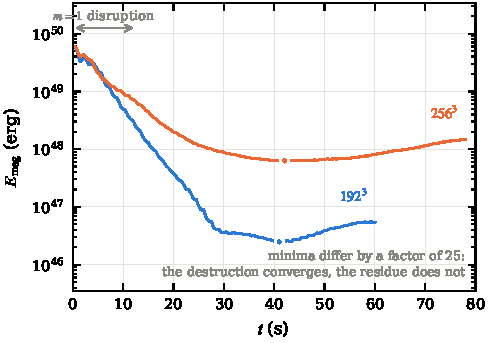
\includegraphics[width=\columnwidth]{figures/fig_decay.pdf}
\caption{Magnetic energy of the star against time on both meshes. The ordered
field loses most of its energy over the first several seconds and the decay
is robust: the two meshes agree on it. Where they do not agree is the level the field settles
to, the minima differing by a factor of $25$, after which the energy rises
again on both. We show both meshes rather than one so that the residue is not
mistaken for a measurement; growth rates and residues are reported as
resolution-limited throughout (Section~\ref{sec:limitations}).
\label{fig:decay}}
\end{figure}

This is the behaviour linear theory predicts for a near-pure toroidal field,
and it is worth being precise about what it does and does not show. It does
not show that toroidal fields cannot exist in white dwarfs; it shows that the
particular branch these equilibrium models are built on is the unstable one.
Section~\ref{sec:limitations} lists the caveats that attach to the measured
growth rate.

\subsection{The stable configuration cannot be evolved in a filled box}

We constructed the twisted-torus counterpart on the identical star --- same
central density, same rotation law, same self-consistent toroidal field, the
poloidal amplitude being the only difference --- and attempted to evolve both.
The control, carrying the literature's weak exterior dipole, ran cleanly to
the target time. The twisted torus aborted at $t = 0.205$~s after a collapse of the time step
(Figure~\ref{fig:probe}), at $35$ times the cost per unit physical time.

\begin{figure}
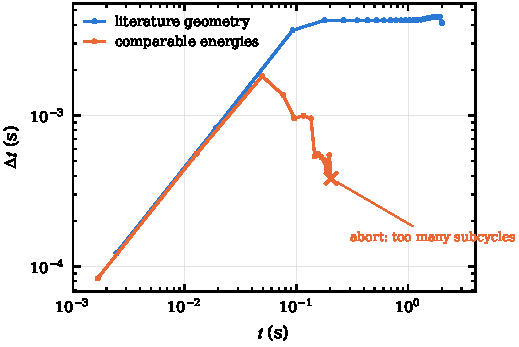
\includegraphics[width=\columnwidth]{figures/fig_probe.pdf}
\caption{Time step against elapsed physical time for the two configurations,
which differ only in poloidal amplitude on an otherwise identical star. Both
ramp identically from the initial reduction. The literature geometry then
holds a step of a few times $10^{-3}$~s and reaches the target time; the
comparable-energy configuration peaks at $t \simeq 0.05$~s and loses the step
in plateaus until the subcycle limit ends the run at $t = 0.205$~s. The pair
is asymmetric by construction --- only one of the two is ambient-limited ---
so the figure shows the constraint of Section~\ref{sec:3d}, not a difference
in stability.
\label{fig:probe}}
\end{figure}

The cause is not numerical fragility but a physical constraint on the setup.
Comparable poloidal energy requires an exterior dipole near $7\times10^{11}$~G.
An ambient medium of $2\times10^{4}$~g~cm$^{-3}$, which is already
$3\%$ of the stellar mass when it fills the domain, holds at most
$3.4\times10^{10}$~G at $\beta = 1$. Raising the ambient to the required
$8.7\times10^{5}$~g~cm$^{-3}$ would put $2.5\,\Msun$ of material in the box,
more than the star. Stronger current confinement does not help: over the
configurations satisfying all four criteria, the Fujisawa localization reduces
the exterior dipole by $8\%$ where a factor of $18$ is needed.

We therefore report this as a result rather than a difficulty. \emph{The
stable branch of magnetized white dwarf equilibria cannot be evolved by a
domain-filling code without a vacuum or stratified exterior treatment}, and
this is a plausible reason why the field has equilibrium models and no
dynamics.

\section{Discussion} \label{sec:discussion}

%% TODO(RL): position against Pakmor & Pelisoli (2024) large-scale dynamo and
%% Becerra et al. (2018) post-merger models; both support the rotational
%% reading.

\subsection{The ceiling coincides with the stability bound}

The ceiling of Section~\ref{sec:ceiling} was obtained from a condition on the
equilibrium: the star must not be asked to carry a field whose pressure
exceeds the gas pressure that the equation of state used to build it was
supplying. It makes no reference to stability. Yet the value it returns,
$\Etor/|W| \le 0.0101$, is the number independently quoted as the bound on
magnetic stability for barotropic stars, $E_{\rm mag}/|W| \simeq 0.01$.

The evolution behaves accordingly. Our production configuration begins at
$E_{\rm mag}/|W| = 0.0114$, marginally above that bound, and the field decays
until the ratio is two orders of magnitude below it, where the decay stops:

\begin{center}
\begin{tabular}{rcc}
\hline
$t$ (s) & $E_{\rm mag}/|W|$ & $\Etor/\Epol$ \\
\hline
 0 & $1.14\times10^{-2}$ & $5\times10^{5}$ \\
 5 & $3.9\times10^{-3}$ & 7.0 \\
12 & $1.4\times10^{-3}$ & 4.2 \\
45 & $1.2\times10^{-4}$ & 77 \\
78 & $2.8\times10^{-4}$ & 89 \\
\hline
\end{tabular}
\end{center}

Read this way the run is not a star losing its field but a star shedding field
until it reaches a configuration it can hold, and then keeping it.

Whether the coincidence of the two numbers is accidental we cannot yet say. A
virial argument suggests it need not be: $|W|$ is of order the volume integral
of the pressure, so $E_{\rm mag}/|W|$ is of order the volume average of
$1/\beta$, and a global energy bound and a local pressure floor would then be
the same statement separated by the ratio between mean and minimum $\beta$.
Establishing that properly is beyond this paper.

\subsection{What the result says}

The results above are consistent and point one way. A white dwarf can hold
only about one per cent of its binding energy in a confined, stably configured
magnetic field. That is twenty times less than the super-Chandrasekhar
equilibrium programme requires, and it is not enough to lift the mass past
degeneracy's own limit. Where a super-Chandrasekhar magnetized white dwarf is
constructible with a stable field geometry, the mass is supplied by
differential rotation and the field is a passenger.

This does not refute the existence of over-massive white dwarfs. It relocates
their support.

\section{Limitations} \label{sec:limitations}

We state these here rather than in a closing paragraph because two of them
bear directly on how the dynamical results should be read.

\textbf{The magnetorotational instability is not resolved, and cannot be.}
With the specified field the fastest-growing MRI wavelength is
$4\times10^{-3}$ of a cell. Resolving it is not a question of cost: the
requirement that the ambient medium hold the field while the MRI wavelength
spans six cells cannot be met by any amplitude within this family. The
literature on merger remnants finds the MRI erasing differential rotation when
it is resolved \citep{pakmor2024}. Our differential rotation survives, and
that outcome is not distinguishable from our simulation being unable to
destroy it.

\textbf{The $m=1$ mode grows on grid noise.} The intended initial poloidal
seed is $\Epol/\Etor = 4.6\times10^{-8}$; the value realized on the mesh is
$1.9\times10^{-6}$, forty times larger, and the difference is discretization
error. The Tayler instability is ideal, so the seed sets the onset time rather
than whether the mode exists, and the growth rate, the $m=1$ character and the
angular-momentum transport are robust to it. The measured growth rate is not:
it rises by $47\%$ from $192^3$ to $256^3$, and the late-time field residue
differs by a factor of $25$ between the same meshes. Growth rates and residues
are reported as resolution-limited.

\textbf{Part of the evolution lies above the critical field.} In the first
twelve seconds, $49\%$ of sampled instants have a peak field exceeding the
Landau critical value, where a field-independent degenerate equation of state
is least defensible. The rotation results, measured from $12$~s onward, are
free of this.

\textbf{Criterion (iii) is imported from stably stratified stars.}
\citet{braithwaite2006} establish the stability of the mixed configuration for
stars with stable stratification. Ours is barotropic, and for barotropes there
is a body of work arguing that no stable magnetic equilibrium exists at all.
Calling the comparable-energy region ``the stable branch'' is therefore a
convenience of language, and criterion (iii) should be read as selecting the
geometry that is stable \emph{where stability is known}, not as asserting
stability here. The relevant control is whether the ordered configuration our
rotating run settles into survives without rotation, since rotation can
stabilize what a barotrope cannot; that run is in progress and will be
reported separately.

\textbf{$\bmin \ge 1$ is a consistency criterion.} It states that the
equilibrium does not contradict the equation of state used to build it. It is
not a stability proof, and only three-dimensional evolution can supply one.

\textbf{The strongly localized corner is not converged.} For
$m \le -1.5$ the survey quantities shift by up to $2.4\%$ in $\bmin$ and
$13\%$ in $\Etor/\Epol$ between $129^2$ and $257^2$, and the shift does not
diminish with refinement. No result reported here draws on that corner: the
configurations satisfying all four criteria use $m = 0$ and $m = -1$, where
the same quantities move by $0.03\%$ and $1\%$ respectively.

\section{Conclusions} \label{sec:conclusions}

\begin{enumerate}
\item A white dwarf holds at most $\Etor/|W| \simeq 0.0101$ in a confined
      toroidal field, nearly independent of central density. The
      super-Chandrasekhar equilibrium programme requires twenty times more.
\item Such a field is worth about $+0.017\,\Msun$. The mass frontier it
      permits converges to $\Mch$ from below and does not cross it, ending at
      neutronization.
\item With differential rotation, twisted-torus configurations above the
      Chandrasekhar mass do exist, reaching $2.13\,\Msun$ at the edge of the
      comparable band and $1.65\,\Msun$ well inside it, but their support
      is rotational and the field still carries about one per cent of the
      virial.
\item The configuration the literature specifies loses $98\%$ of its
      magnetic energy to an $m=1$ instability in a few Alfv\'en times, as
      linear theory predicts for a near-pure toroidal field. The field stays
      ordered and axisymmetric; it is the $10^{14}$~G amplitude that does not
      survive.
\item The stable alternative cannot be evolved in a domain-filling code:
      comparable poloidal energy implies an exterior dipole that no affordable
      ambient medium confines.
\end{enumerate}

\begin{acknowledgments}
%% TODO(RL): CENAPAD acknowledgment in their required wording.
The authors acknowledge the use of computational resources from the
\href{https://computacaocientifica.ufes.br/scicom}{Sci-Com Lab} of the
Department of Physics at UFES, supported by FAPES, CAPES, and CNPq.
\end{acknowledgments}

\software{CASTRO \citep{almgren2010}, AMReX \citep{zhang2019},
          NumPy \citep{harris2020}, SciPy \citep{virtanen2020}}

\bibliography{refs}
\bibliographystyle{aasjournal}

\end{document}
